\subsection*{Q3 - [30 points]}

\begin{solution}
    \begin{parts}
        \part The value of $r_s$ should be -1 for the optimal policy to return the shortest path to the target square, as the agent would be penalized by -1 for each step taken if its not the target square. This would ensure that the agent takes the shortest path to the target square.
        
        We can then use Bellman's equation to find the optimal equation for the target square, which is:

        $$ v(s) = \max_{a \in A(s)} \displaystyle\sum_{s', r} p(s', r \mid s, a)[r + \gamma v(s')] $$

        Since the transition is deterministic, so there is no ``probability'' of the agent landing on any other square other than intended, we can simplify this to:
        \begin{align*}
            v(s) &= \max_{a \in A(s)}[r + \gamma v(s')] \\
            &= \max_{a \in A(s)}[-1 + v(s')] \hspace*{10mm} \because \gamma = 1\\
        \end{align*}

        Since the agent is penalized by -1 for each step taken, the optimal policy would be to take the action that maximizes the value of $v(s)$, which is to move to the target square.
        
        The image below shows the optimal values from each square:
        \begin{figure}[H]
            \centering
            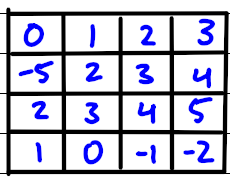
\includegraphics[width=0.25\textwidth]{q3_a.png}
        \end{figure}

        % \part Value function $ V_\pi \text{old}(s) = \E $
        \part Given a general MDP, rewards increase by $ r' = r + c $

        The value function is $ V_\pi \text{old}(s) $

        Then the new value function can be defined as: 

        \begin{align*}
            V_\pi \text{new}(s) &= \displaystyle\sum_{t = 0}^{\infty} \gamma^tr'(s_t) \\
            &= V_\pi \text{old}(s) + \displaystyle\sum_{t = 0}^{\infty} \gamma^tc
        \end{align*}
        where the old value function can be defined as $ V_\pi \text{old}(s) = \displaystyle\sum_{t = 0}^{\infty} \gamma^tr(s_t) $

        Since the horizon in infinite, then it becomes an infinite gemetric series as so:
        $$ \displaystyle\sum_{t = 0}^{\infty}\gamma^tc = \displaystyle\frac{c}{1 - \gamma}, \hspace*{10mm} \text{if} \mid \gamma \mid < 1 $$
        
        Thus, the new value function becomes:
        $$ V_\pi \text{new}(s) = V_\pi \text{old}(s) + \displaystyle\frac{c}{1 - \gamma} $$

        \part If we increase the value of $r_s$ to +2, and $ c = 3 $, then $ r_g = 5 + 3 = 8 $, and $ r_r = -2 $.

        Then the our new values become:

        \begin{figure}[H]
            \centering
            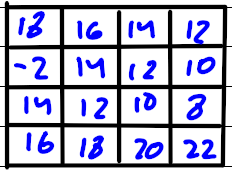
\includegraphics[width=0.25\textwidth]{q3_c.png}
        \end{figure}

        The above grid is only assuming that the agent follows the same optimal path from the first part. In reality, since the agent's reward is getting +2 for each non-terminal square, it would be more beneficial for the agent to take the longest path to the target square, as it would get more rewards. This could result in the agent getting stuck on squares 6, 7, 10 and 11 indefinitely as they would perpetually increase the agent's reward. 
    \end{parts}
\end{solution}